\documentclass[11pt]{cernrep}
\usepackage{graphicx,epsfig}
\bibliographystyle{lesHouches}

\usepackage{xspace}
\newcommand{\Sherpa}{S\protect\scalebox{0.8}{HERPA}\xspace}
\newcommand{\Powheg}{P\protect\scalebox{0.8}{OWHEG}\xspace}
\newcommand{\CSS}{C\protect\scalebox{0.8}{SS}\xspace}
\newcommand{\Comix}{C\protect\scalebox{0.8}{OMIX}\xspace}
\newcommand{\Amegic}{A\protect\scalebox{0.8}{MEGIC++}\xspace}
\newcommand{\MCatNLO}{M\protect\scalebox{0.8}{C}@N\protect\scalebox{0.8}{LO}\xspace}
\newcommand{\MEPS}{M\scalebox{0.8}{E}P\scalebox{0.8}{S}\xspace}
\newcommand{\MEPSatNLO}{M\scalebox{0.8}{E}P\scalebox{0.8}{S}@N\protect\scalebox{0.8}{LO}\xspace}
\newcommand{\Collier}{C\protect\scalebox{0.8}{OLLIER}\xspace}
\newcommand{\OpenLoops}{O\protect\scalebox{0.8}{PEN}L\protect\scalebox{0.8}{OOPS}\xspace}
\newcommand{\Herwig}{H\protect\scalebox{0.8}{ERWIG}7\xspace}
\newcommand{\Matchbox}{M\protect\scalebox{0.8}{ATCHBOX}\xspace}
\newcommand{\MGaMC}{M\protect\scalebox{0.8}{AD}G\protect\scalebox{0.8}{RAPH}5\_aMC@NLO\xspace}
\newcommand{\MadGraph}{M\protect\scalebox{0.8}{AD}G\protect\scalebox{0.8}{RAPH}\xspace}
\newcommand{\MadGraphfour}{M\protect\scalebox{0.8}{AD}G\protect\scalebox{0.8}{RAPH}4\xspace}
\newcommand{\CVolver}{CV\protect\scalebox{0.8}{OLVER}\xspace}
\newcommand{\ColorFull}{C\protect\scalebox{0.8}{OLOR}F\protect\scalebox{0.8}{ULL}\xspace}
\newcommand{\MoCaNLO}{M\protect\scalebox{0.8}{oCaNLO}\xspace}
\newcommand{\Recola}{R\protect\scalebox{0.8}{ecola}\xspace}
\newcommand{\pt}{\ensuremath{p_{T}}\xspace}
\newcommand\sss{\mathchoice%
{\displaystyle}%
{\scriptstyle}%
{\scriptscriptstyle}%
{\scriptscriptstyle}%
}
\newcommand\MSB{\ifmmode {\overline{\rm MS}} \else $\overline{\rm MS}$\fi}
\newcommand\MINLO{{\tt MiNLO}}
\newcommand\muf{\mu_{\sss\rm F}}
\newcommand\mur{\mu_{\sss\rm R}}
\newcommand\KRA{K_{\scriptscriptstyle \rm R}}
\newcommand\KFA{K_{\scriptscriptstyle \rm F}}

\newcommand{\GOSAM}{G\protect\scalebox{0.8}{O}S\protect\scalebox{0.8}{AM}\xspace}
\newcommand{\POWHEGBOX}{P\protect\scalebox{0.8}{OWHEG} B\protect\scalebox{0.8}{OX}\xspace}
\newcommand{\QGRAF}{Q\protect\scalebox{0.8}{GRAF}\xspace}
\newcommand{\FORM}{F\protect\scalebox{0.8}{ORM}\xspace}
\newcommand{\SAMURAI}{S\protect\scalebox{0.8}{AMURAI}\xspace}
\newcommand{\GOLEM}{G\protect\scalebox{0.8}{OLEM}\xspace}
\newcommand{\NINJA}{N\protect\scalebox{0.8}{INJA}\xspace}
\newcommand{\SPINNEY}{S\protect\scalebox{0.8}{PINNEY}\xspace}
\newcommand{\ONELOOP}{O\protect\scalebox{0.8}{NE}LO\protect\scalebox{0.8}{OP}\xspace}
\newcommand{\MCFM}{M\protect\scalebox{0.8}{CFM}\xspace}

% Commands defined by Mathieu
\usepackage{amsmath}
\newcommand{\MP}[1]{{ {\color{blue}{ [MP: #1]}} }}

\usepackage{color}
\usepackage{morefloats}

\begin{document}

\section{Study of electroweak production of WZ in association with two
  jets at the LHC \protect\footnote{Section
    coordinators: K.~D.~Long, M.~Pellen}$^{,}$ \protect\footnote{Contributing authors:
    S.~Br\"auer, V.~Ciulli, M.~Herndon, S.~Gieseke, M.~Mozer, S.~Pl{\"a}tzer,
    M.~Rauch, E.~Yazgan.}$^{,}$
  \protect\footnote{{\it next some examples of acknowledgements}}$^{,}$
  \protect\footnote{ A. Aaaaa acknowledges support by a FP7 Marie
    Curie Intra European Fellowship under Grant Agreement xxxx.}$^{,}$
\protect\footnote{The work of B. Bbbb is supported in part by the
  U.S. Department of Energy under grant yyyy.} \label{vbs_section}}

\subsection{Introduction \label{vbs_intro}}

The electroweak (EW) production of vector-boson pairs in association with two jets at the CERN Large Hadron Collider (LHC) represents a very important type of processes both theoretically and experimentally.
This class of processes is dominated by vector-boson scattering (VBS) contributions and constitutes thus the first type of processes where the scattering of two massive gauge bosons can be observed at the LHC.
In the scattering of two massive gauge bosons, the Higgs boson is playing a very special role.
It prevents the cross section from diverging in the high-energy limit and preserve the unitarity of the associated scattering amplitude.
More importantly, these vector-boson scattering (VBS) signatures just started to be observed and even measured by the experimental collaborations at the LHC.
These are particularly challenging measurement to the high multiplicity of the processes and their small cross sections.
The best measurement \cite{Aad:2014zda,Khachatryan:2014sta,Sirunyan:2017ret,Aaboud:2016ffv} concerns the signature where the scattering of same sign W boson occurs (usually denoted ${\rm W}^\pm{\rm W}^\pm{\rm j}{\rm j}$).
The reason for this is that is posses a very specific structure due to the same sign charged leptons in the final state.
Therefore, in addition to have a rather large cross section, it also possesses a low irreducible background.
Other signature such as ${\rm Z}{\rm Z}{\rm j}{\rm j}$, ${\rm W}^+{\rm W}^-{\rm j}{\rm j}$, or ${\rm W}^{\pm}{\rm Z}{\rm j}{\rm j}$ are even more challenging due to the lower cross section and large irreducible background.
Nonetheless, observations have already been performed at the LHC for both the ZZ \cite{CMS-PAS-SMP-16-019} and WZ \cite{Aad:2016ett} scattering \MP{Experimental references to be added/modified.}.

From a theoretical point of view, one of the challenges for the predictions of the EW di-boson production in association with two jets is its high multiplicity.
This explains why in the past, next-to-leading order (NLO) predictions have focused on VBS approximations.
Only recently, full NLO computations became available at NLO QCD and EW for both the EW component and the QCD-induced process for ${\rm W}^\pm{\rm W}^\pm{\rm j}{\rm j}$ \cite{Biedermann:2017bss}.
For this process, preliminary results \cite{Anders:2018gfr} of a comparison of different theoretical predictions have shown that differences between the full computation and VBS-approximate ones are not significant given the present experimental accuracy.
Qualitatively, one could expect a similar conclusion for other processes such as WZ.
Note that this only a qualitative statement.
Indeed, the ${\rm W}^{\pm}{\rm Z}{\rm j}{\rm j}$ process possesses more non-VBS contributions making VBS approximations more likely to be inaccurate.

An experimental challenge is the presence of an irreducible background.
It is of order $\mathcal{O} (\alpha_{\rm s}^2 \alpha)$ and is usually dubbed QCD-induced process.
\MP{Some extra comments on the specific experimental challenges to measure WZ.}

Therefore a preliminary study aiming at comparing various approximations and predictions used in the literature is particularly well motivated.
The present study focus on leading-order (LO) predictions (possibly supplied with a parton shower) with realistic experimental event selection.
\MP{Explain what we do here depending on what we have.}

In particular, the study focuses on two partonic processes

\begin{equation}
 {\rm p} {\rm p} \to {\rm e}^+  \nu_{\rm e}  \mu^+ \mu^- {\rm j} {\rm j} ,
\end{equation}
%
and
%
\begin{equation}
 {\rm p} {\rm p} \to {\rm e}^-  \bar \nu_{\rm e}  \mu^+ \mu^- {\rm j} {\rm j},
\end{equation}
%
at order $\mathcal{O} (\alpha^6)$.


\subsection{Theory and event generators \label{vbs_theory}}

This study focuses on LO predictions but NLO QCD corrections to the EW contribution and its irreducible background are already known.
The QCD corrections to the EW contributions are known since 10 years in the VBS approximation \cite{Bozzi:2007ur} while the QCD corrections to the QCD-induced process has been computed more recently \cite{Campanario:2013qba}.
The NLO EW corrections are currently unknown.
In Ref.~\cite{Biedermann:2016yds}, it has been argued that large NLO EW corrections to the EW contributions are an intrinsic feature of VBS at the LHC.
Therefore, they are expected to play a significant role for all VBS signatures.
In Ref.~\cite{Biedermann:2017bss}, which focuses on the computation of the full NLO corrections to the ${\rm W}^\pm{\rm W}^\pm{\rm j}{\rm j}$ process, it has been shown that the EW corrections to the EW process are the dominant NLO corrections.
This means that the EW corrections to the EW contributions are expected to be at least of the same order than the QCD ones for VBS signatures.
\MP{Add some comments on parton shower effects that can play a significant role.}

{\it Add here a description of the theory tools and generators
  used. Below there are same short samples taken from previous proceedings.}

\subsubsection*{\Herwig \label{vbs_herwig}}
\MP{This subsubsection is out-dated I think. Isn't it?}

In this section we present the setup for those results obtained with the
\Herwig event generator~\cite{Bellm:2015jjp,Bahr:2008pv}.

Based on extensions of the previously developed \Matchbox
module~\cite{Platzer:2011bc}, \Herwig facilitates the automated setup of all
ingredients necessary for a full NLO QCD calculation in the subtraction
formalism: an implementation of the Catani--Seymour dipole subtraction
method~\cite{Catani:1996vz,Catani:2002hc}, as well as interfaces to a list of
external matrix--element providers -- either at the level of squared matrix
elements, based on extensions of the BLHA
standard~\cite{Binoth:2010xt,Alioli:2013nda,Andersen:2014efa}, or at the
level of color--ordered subamplitudes, where the color bases are provided by
an interface to the \ColorFull~\cite{Sjodahl:2014opa} and
\CVolver~\cite{Platzer:2013fha} libraries.

For this study the relevant tree--level matrix elements etc, etc... 

The PDF sets being used are MMHT2014lo68cl and
MMHT2014nlo68cl~\cite{Harland-Lang:2014zoa}, i.e. the default PDF sets
to which the showers are currently tuned.

\subsubsection*{\protect\Sherpa \label{vbs_sherpa}}
In this section we present the setups that are used in this study for the \Sherpa event
generator~\cite{Gleisberg:2008ta}. 
Etc, etc... 

\subsubsection*{\protect{\MoCaNLO\!+\Recola} \label{vbs_MoCaNLO_Recola}}

The program {\sc MoCaNLO+Recola} is made of a flexible Monte Carlo program dubbed {\sc MoCaNLO} and of the general matrix element generator {\sc Recola}~\cite{Actis:2012qn,Actis:2016mpe}.
The program can compute arbitrary processes in the Standard Model with NLO QCD and EW accuracy.
The fast integration is ensured by using similar phase-space mappings to those of Refs.~\cite{Berends:1994pv,Denner:1999gp,Dittmaier:2002ap}.
The IR divergences appearing in the real corrections are handles with the help of the Catani--Seymour dipole formalism \cite{Catani:1996vz,Dittmaier:1999mb}.
To numerically evaluate the one-loop scalar and tensor integrals, {\sc Recola} relies on the {\sc Collier} library \cite{Denner:2014gla,Denner:2016kdg}.
Note that the complex-mass scheme~\cite{Denner:1999gp,Denner:2005fg} to treat unstable particles is always used.
These tools have been successfully used for the computation of NLO corrections for high-multiplicity processes and in particular VBS processes \cite{Biedermann:2016yds,Biedermann:2017bss}.

\subsection{Experimental analysis \label{vbs_rivet}}

Results in this study were produced using a Rivet routine that
mimics ATLAS and CMS preliminary analyses. Distributions include the number of jets, etc,...

\subsubsection*{Input parameters}

All simulation are performed for the LHC running with a center-of-mass energy $\sqrt s = 13 {\rm TeV}$.
The default parton density function (PDF) used is the NNPDF~3.0 set~\cite{Ball:2014uwa} with four active flavour at LO and a strong coupling constant $\alpha_{\rm s}\left( M_{\rm Z} \right) = 0.130$.\footnote{Its {\tt lhaid} in LHAPDF6~\cite{Buckley:2014ana} is 263400.} 
% NNPDF30_lo_as_0130_nf_4 
If this default PDF is not employed, it is explicitly stated.

The masses and widths of the particle used in the simulations are
%
\begin{alignat}{2}
                M_{\rm t}   &=  173.21 {\rm GeV},             & \quad \quad \quad \Gamma_{\rm t} &= 0 {\rm GeV},  \nonumber \\
                M_{\rm Z}^{\rm OS} &=  91.1876{\rm GeV},      & \quad \quad \quad \Gamma^{\rm OS}_{\rm Z} &= 2.4952{\rm GeV},  \nonumber \\
                M_{\rm W}^{\rm OS} &=  80.385{\rm GeV},       & \Gamma^{\rm OS}_{\rm Z} &= 2.085{\rm GeV},  \nonumber \\
                M_{\rm H} &=  125.0{\rm GeV}, 		      & \Gamma_{\rm H}   &=  4.07 \times 10^{-3}{\rm GeV}.
\end{alignat}
%
The numerical values used in the simulation for the pole mass/width of the gauge bosons ($V={\rm W,Z}$) are obtained from the measured on-shell (OS) values for the masses and widths according to Ref.~\cite{Bardin:1988xt} as:
%
\begin{equation}
        M_V = M_{\rm V}^{\rm OS}/\sqrt{1+(\Gamma_{\rm V}^{\rm OS}/M_{\rm V}^{\rm OS})^2}\,,\qquad  \Gamma_V = \Gamma_{\rm V}^{\rm OS}/\sqrt{1+(\Gamma_{\rm V}^{\rm OS}/M_{\rm V}^{\rm OS})^2}.
\end{equation}

%
The EW coupling is renormalised in the $G_\mu$ scheme \cite{Denner:2000bj} where
%
\begin{equation}
    G_{\mu}    = 1.16637\times 10^{-5}{\rm GeV}^{-2}.
\end{equation}
%
With the previous input parameters, it corresponds to a numerical value for $\alpha$ of
%
\begin{equation}
 \alpha = 7.555310522369 \times 10^{-3}.
\end{equation}
%
Note that for the EW contribution of order $\mathcal{O} (\alpha^6)$, no dependence on the strong coupling appears.
For contributions (interference or QCD-induced contributions) where there is a dependence on $\alpha_{\rm s}$, the numerical value used is the one (potentially dynamically) extracted from the PDF set.

The renormalisation and factorisation scales are set dynamically to \MP{We might have to adapt this depending on the results we show results for fixed scale.}
%
\begin{equation}
\label{eq:defscale}
 \mu_{\rm ren} = \mu_{\rm fac} = {\rm Max}\left[p_{\rm T, j}\right],
\end{equation}
%
which should be understood as the maximum of the transverse momenta of the tagging jets (defined below).
\MP{Justification for this scale choice?}

Photon-induced as well as bottom induced contributions have been neglected.
The photon contributions are expected to be small \cite{Biedermann:2017bss} while the bottom induced contribution can lead to single-top resonant contributions.

\subsubsection*{Event selection}

Following experimental studies \cite{Aad:2016ett,CMS-PAS-SMP-14-008}, the event selection used for the present work is:

\begin{itemize}
\item All charged leptons are required to have
    \begin{align}
        \label{cut:1}
         p_{\rm T, \ell} >  20{\rm GeV},\qquad |y_{\ell}| < 2.5.
    \end{align}
\item For the leptons of opposite charge and same flavour, an invariant mass cut to single out the Z-boson resonance is applied:
    \begin{align}
        \label{cut:2}
         76 {\rm GeV} < m_{l_i^+ l_i^-} < 106 {\rm GeV}.
    \end{align}

\item QCD jets are clustered thanks to the anti-$k_T$ algorithm~\cite{Cacciari:2008gp} with radius parameter $R=0.4$.
      At least two jets are required to have
        \begin{align}
        \label{cut:3}
         p_{\rm T, j} >  30{\rm GeV}, \qquad |y_{\rm j}| < 4.7, \qquad \Delta R_{\rm j \ell} > 0.4,
        \end{align}
        %
        and are called tagging jets.
\item On the two leading tagging jets, typical VBS cuts are applied:
        \begin{align}
        \label{cut:4}
         m_{\rm j j} >  500{\rm GeV},\qquad |\Delta y_{\rm j j}| > 2.5.
        \end{align}
\end{itemize}

\subsection{Results \label{vbs_results}}

\subsubsection*{Cross sections}

\subsubsection*{Differential distributions}

The plot in Figure~\ref{vbs_fig1} etc... 

\begin{figure}[htbp]
\begin{center}
   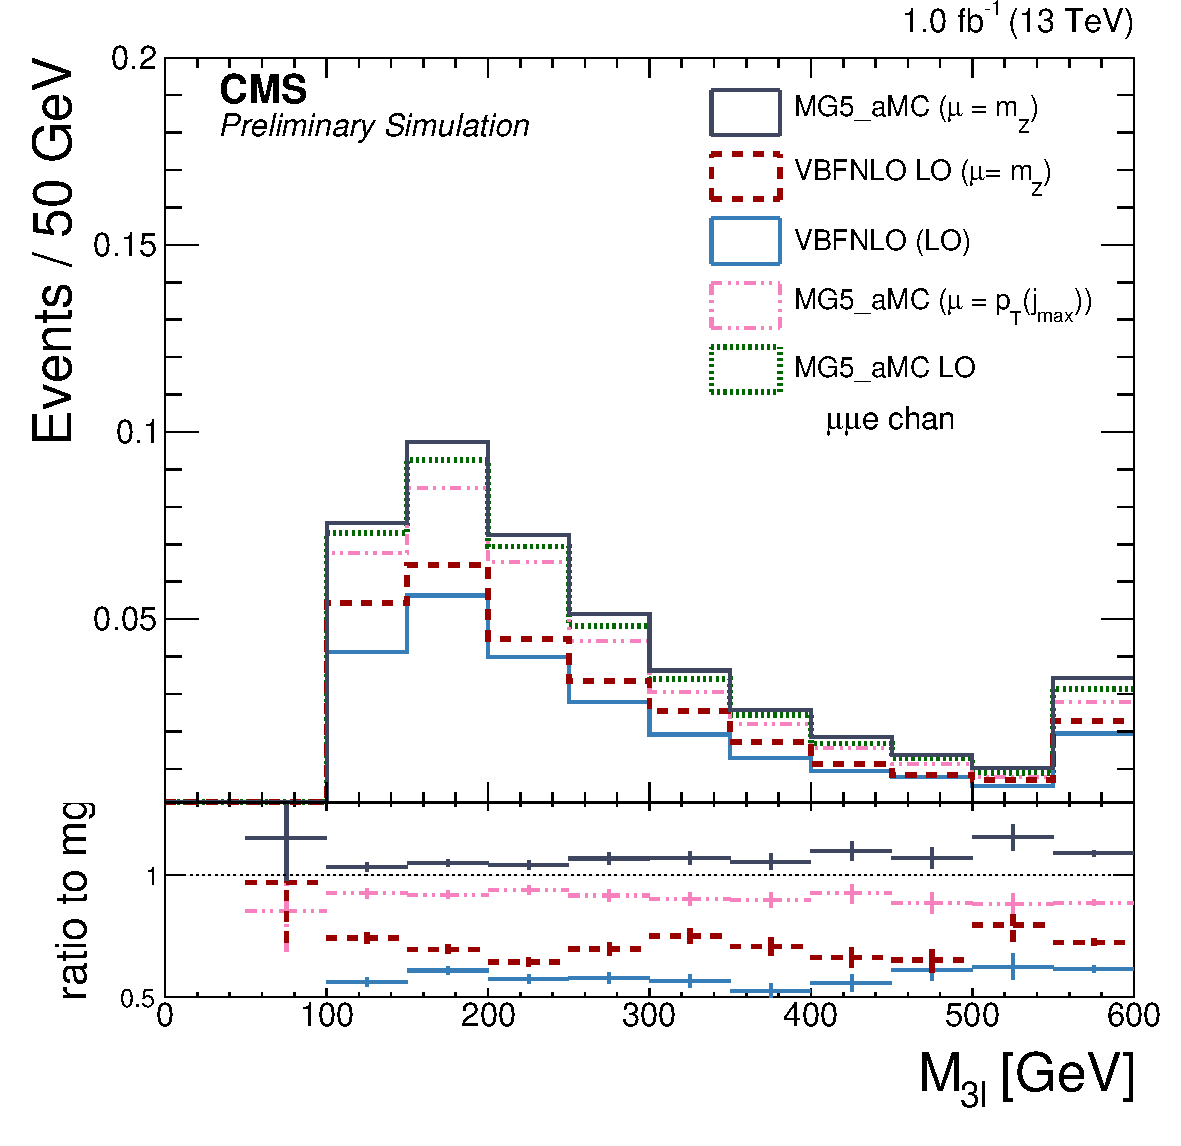
\includegraphics[scale=0.65]{figs/3lmass.pdf}
\caption{A placeholder...}
\label{vbs_fig1}
\end{center}
\end{figure}

\subsection{Conclusions \label{concl}}

We presented a comparison of LO predictions for ${\rm W}^{\pm}{\rm Z}{\rm j}{\rm j}$.
These are implemented on different Monte Carlo programs or generators.
We emphasis that this is a \emph{tuned} comparison where special care had taken to try to match all inputs of these programs.

Significant differences in the predictions can arise from different choices of inputs and no actual physical meaning.

electroweak production of WZ in association with two jets at the LHC, etc... 

Overall these results show that etc...

%\clearpage
\bibliography{vbs_bib}

\end{document}
